\chapter{Anhang}
\label{ch:anhang}

\section{Lösungsansatz}
\label{sec:anhang-loesungsansatz}

\begin{figure}[htb]
\centering
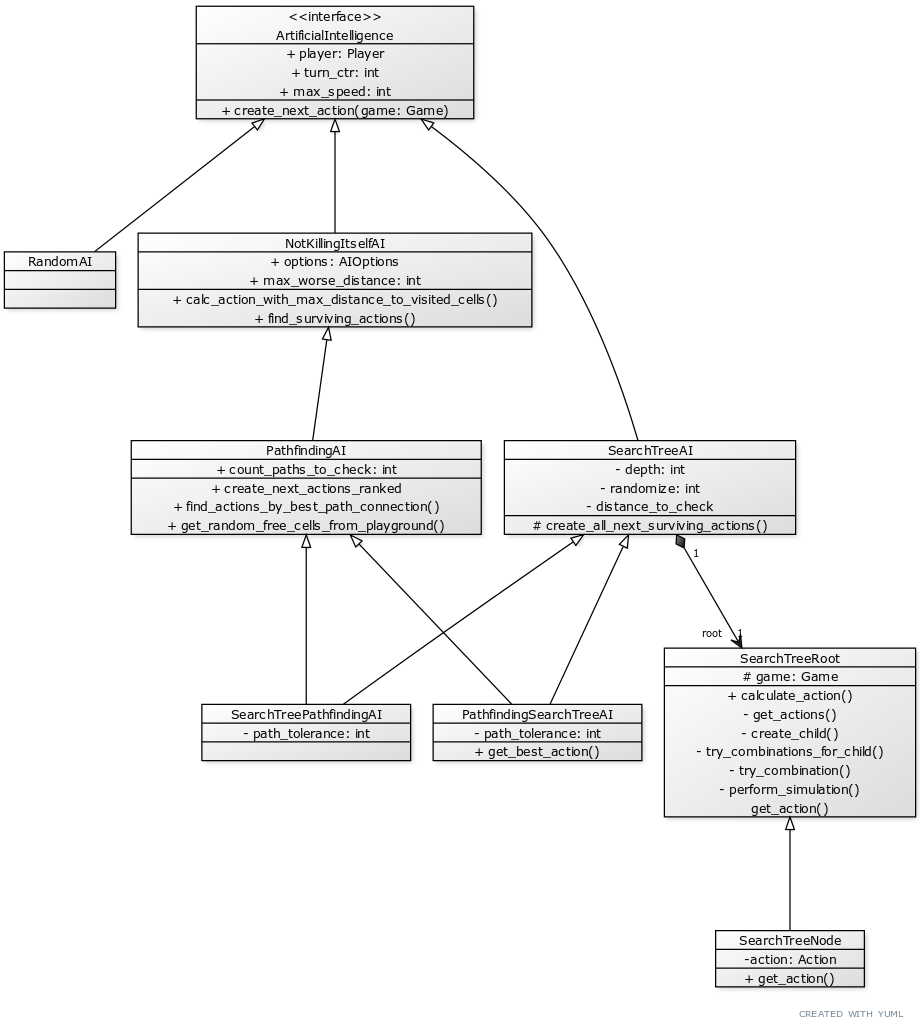
\includegraphics[width=0.8\textwidth]{Bilder/Klassendiagramm_AIs.png}
\caption{UML-Klassendiagramm der \ac{KI}s}
\label{fig:klassendiagramm-AIs}
\end{figure}

\begin{figure}[htb]
\centering
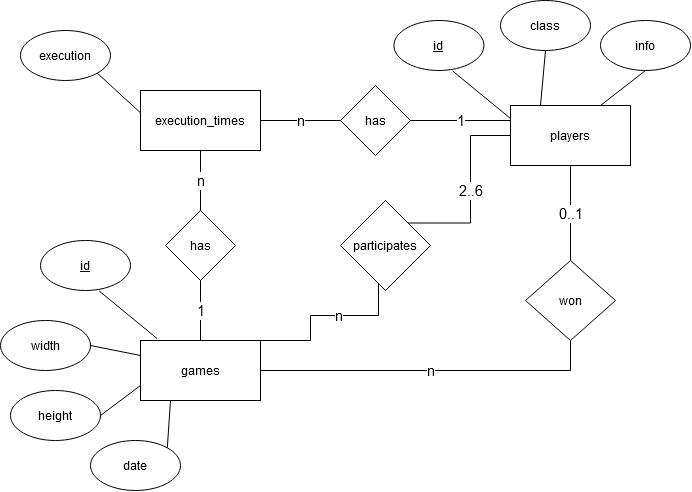
\includegraphics[width=0.8\textwidth]{Bilder/er-diagram.png}
\caption{Entity-Relationship-Modell der Evaluations-Datenbank}
\label{fig:er-schema}
\end{figure}

\begin{figure}[htb]
\centering
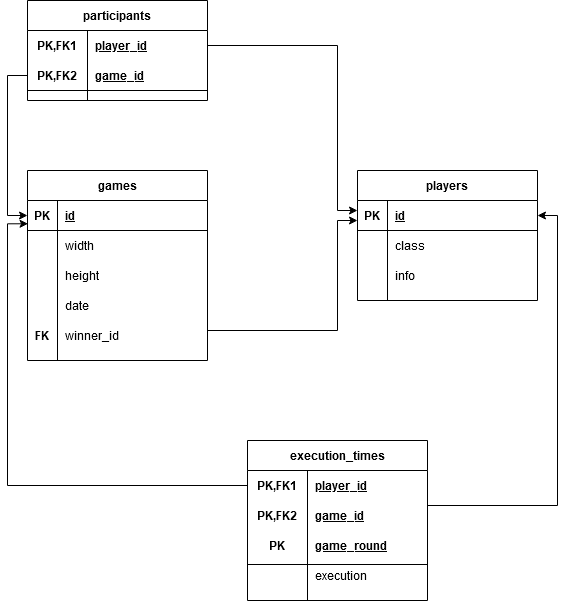
\includegraphics[width=0.8\textwidth]{Bilder/relationales_db_schema.png}
\caption{Relationales Datenbankschema der Evaluations-Datenbank}
\label{fig:relationales-db-schema}
\end{figure}

\section{Implementierung}
\label{sec:anhang-implementierung}

\begin{figure}[htb]
	\centering
	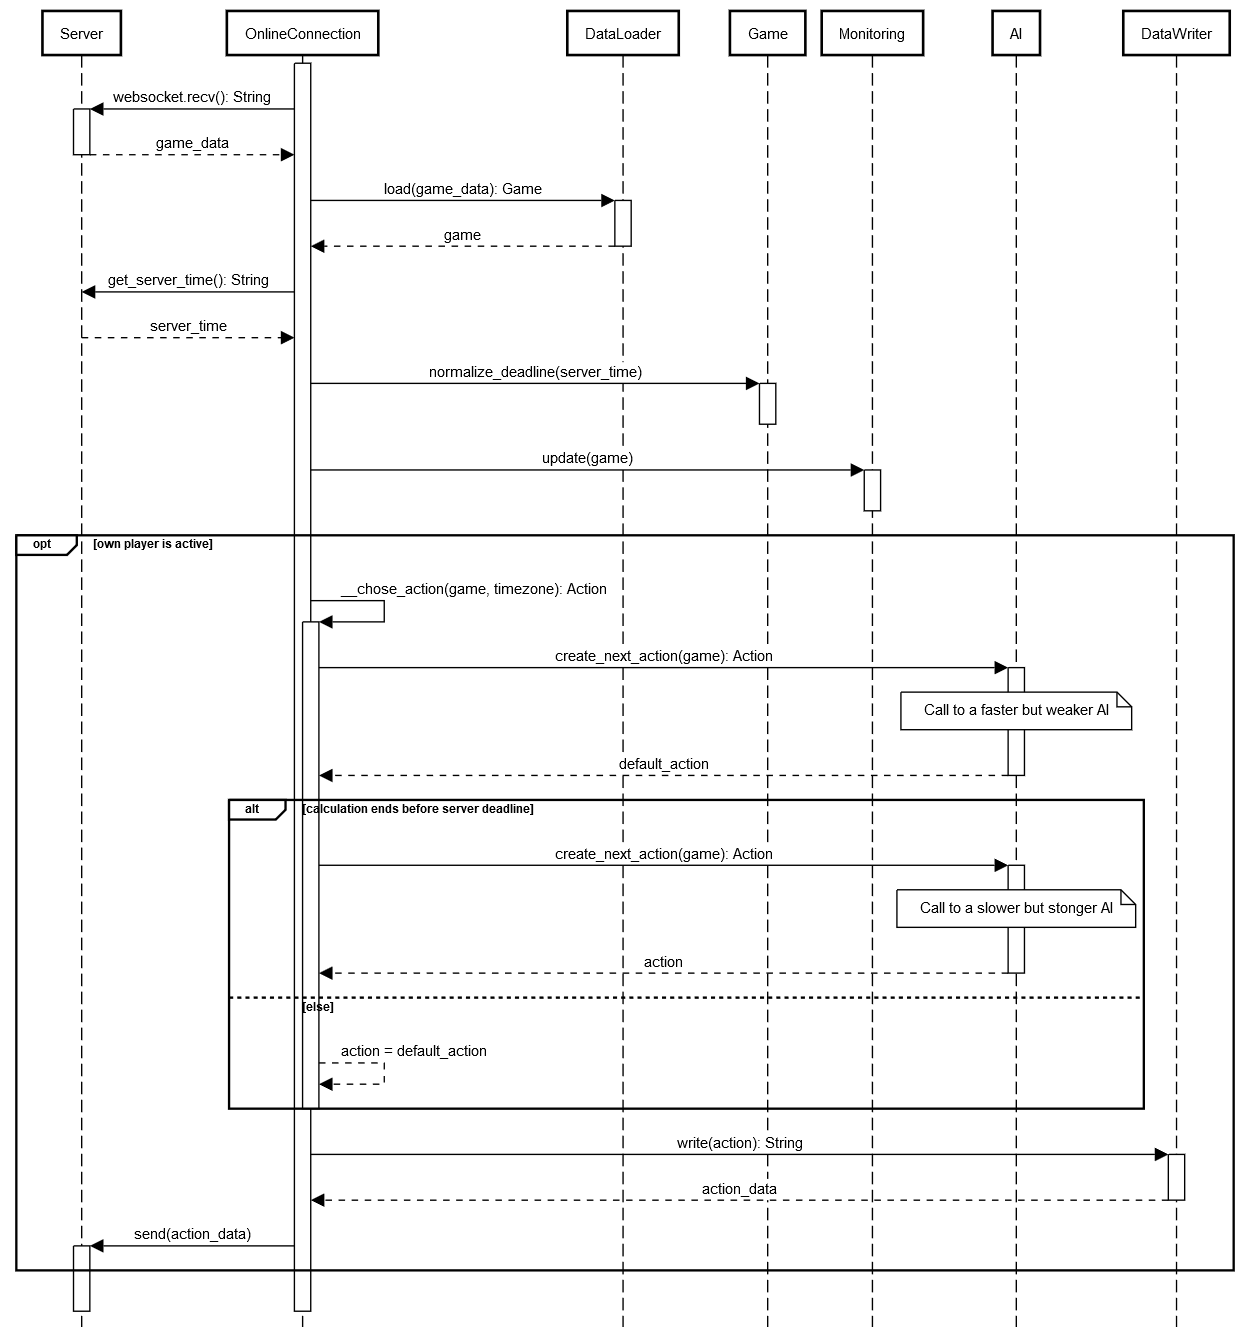
\includegraphics[width=\textwidth]{Bilder/Sequenzdiagramm_Implementierung_Spielzug.png}
	\caption{Sequenzdiagramm zur Implementierung eines Spielzug}
	\label{fig:sequenzdiagramm-spielzug}
\end{figure}

\begin{minipage}{\textwidth}
	\lstinputlisting[label=lst:online-__play,language=Python,caption=\Code{\_\_play()}-Methode des \Code{OnlineController}s]
	{./Dokumente/OnlineController-__play.txt}
\end{minipage}

\begin{minipage}{\textwidth}
	\lstinputlisting[label=lst:json-spiel,language=JSON,caption=JSON-Repräsentation eines Spiel-Zustands]
	{../tests/test_data/ai/game_2.json}
\end{minipage}

\begin{figure}[htb]
	\centering
	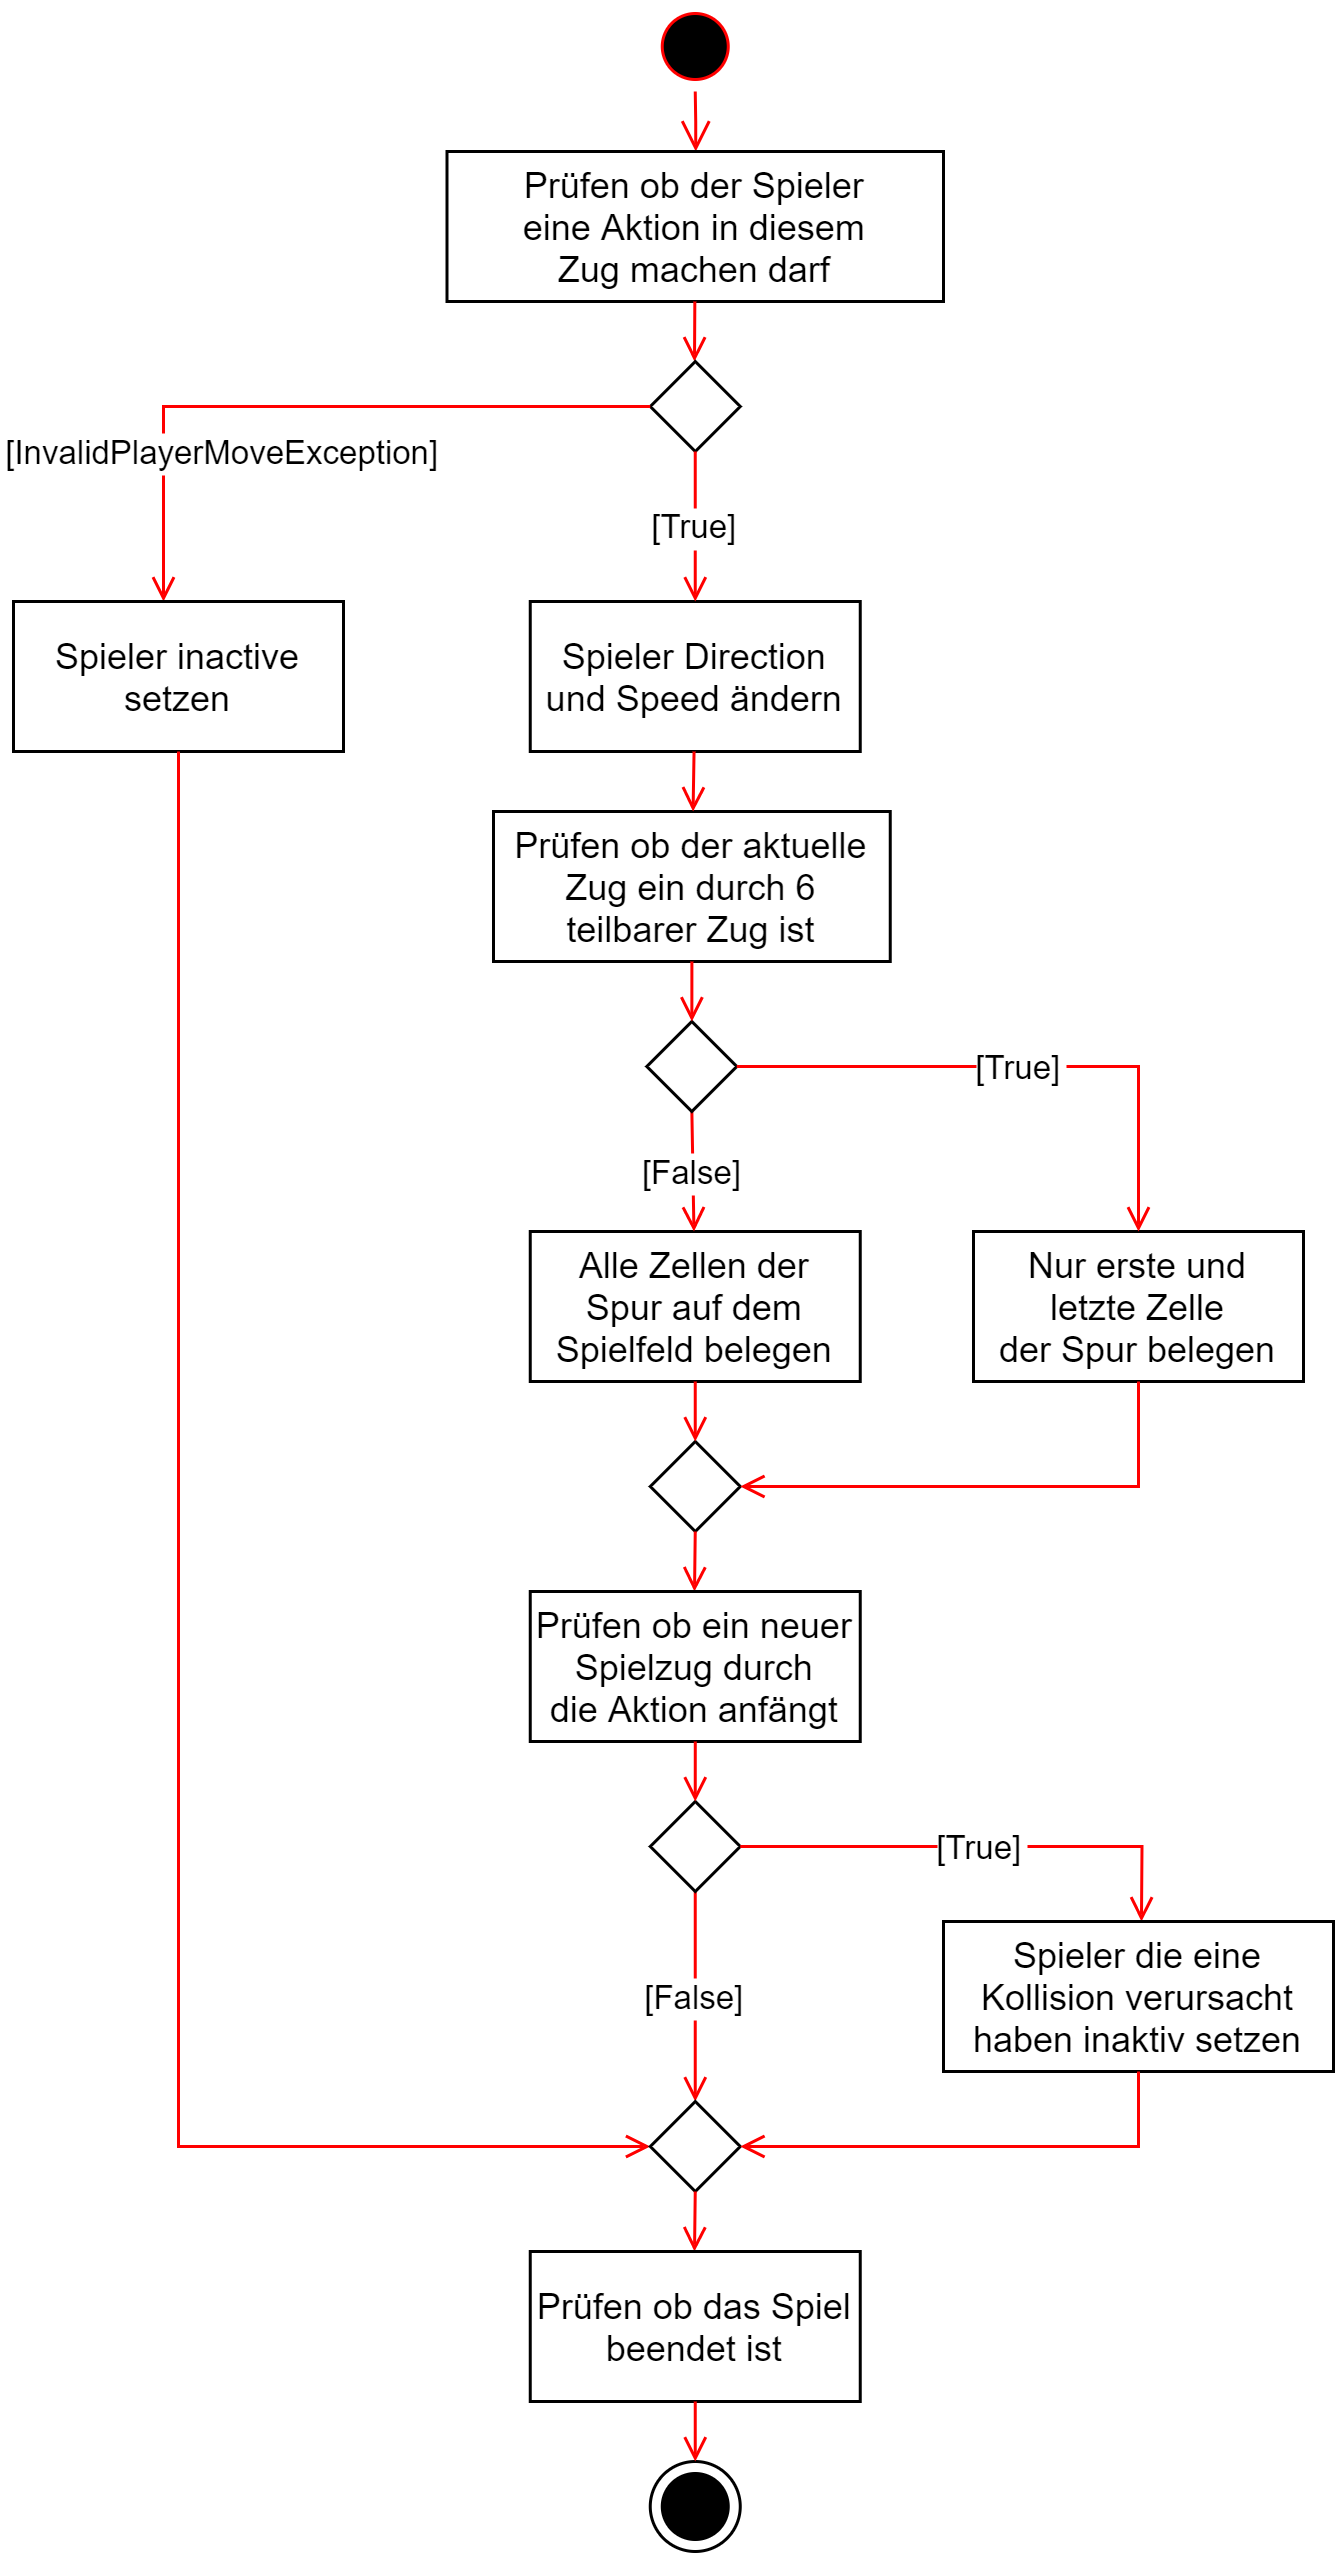
\includegraphics[width=0.7\textwidth]{Bilder/game_service_do_action_activity_diagram.png}
	\caption{Aktivitätsdiagramm zur Durchführung einer Spieler-Aktion durch den \Code{GameService}}
	\label{fig:aktivitaetsdiagramm-spieleraktion-gameservice}
\end{figure}

\begin{minipage}{\textwidth}
	\lstinputlisting[label=lst:get-and-visit-cells
	,language=Python,caption=\Code{get\_and\_visit\_cells(player, action)}-Methode des \Code{GameService}]
	{./Dokumente/Get_And_Visit_Cells_GameService.txt}
\end{minipage}

\begin{minipage}{\textwidth}
	\lstinputlisting[label=lst:pygame_update
	,language=Python,caption=\Code{update(game: Game)}-Methode der \Code{GraphicalView}]
	{./Dokumente/graphicalview_update.txt}
\end{minipage}

\section{Weiterentwicklung}
\label{sec:anhang-weiterentwicklung}

\begin{minipage}{\textwidth}
	\lstinputlisting[label=lst:yaml-github-action,language=YAML,caption=YAML-Konfiguration der Github Action]
	{../.github/workflows/python-app.yml}
\end{minipage}
